%\chapter{Symbole przyjęte w pracy}
%\label{app:symbole}

%Jeśli w tekście nie wykazano inaczej, stosowane symbole należy rozumieć jako:

%\begin{itemize}
%\item[$f(x,y)$] - jasność piksela o współrzędnych $(x,y)$ w obrazie wejściowym,
%\item[$g(x,y)$] - jasność piksela o współrzędnych $(x,y)$ w obrazie wynikowym,
%\item[$t$, $t_i$] - wartości progowe,
%\item[$G$] - liczba poziomów szarości obrazu; $G=256$,
%\item[$P(i,j)$] - macierz GLCM,
%\item[$M(i,j)$] - maska przetwarzania.
%\end{itemize}


%%%%%%%%%%%%%%%%%%%%%%%%%%%%%%%%%%%%%%%%%%%%%%%%%%%%%%%%
\chapter{AchillesDL: System komputerowego wspomagania oceny gojenia ścięgien i więzadeł}
\label{app:AchillesDL}
\begin{figure}[H]
	\centering
	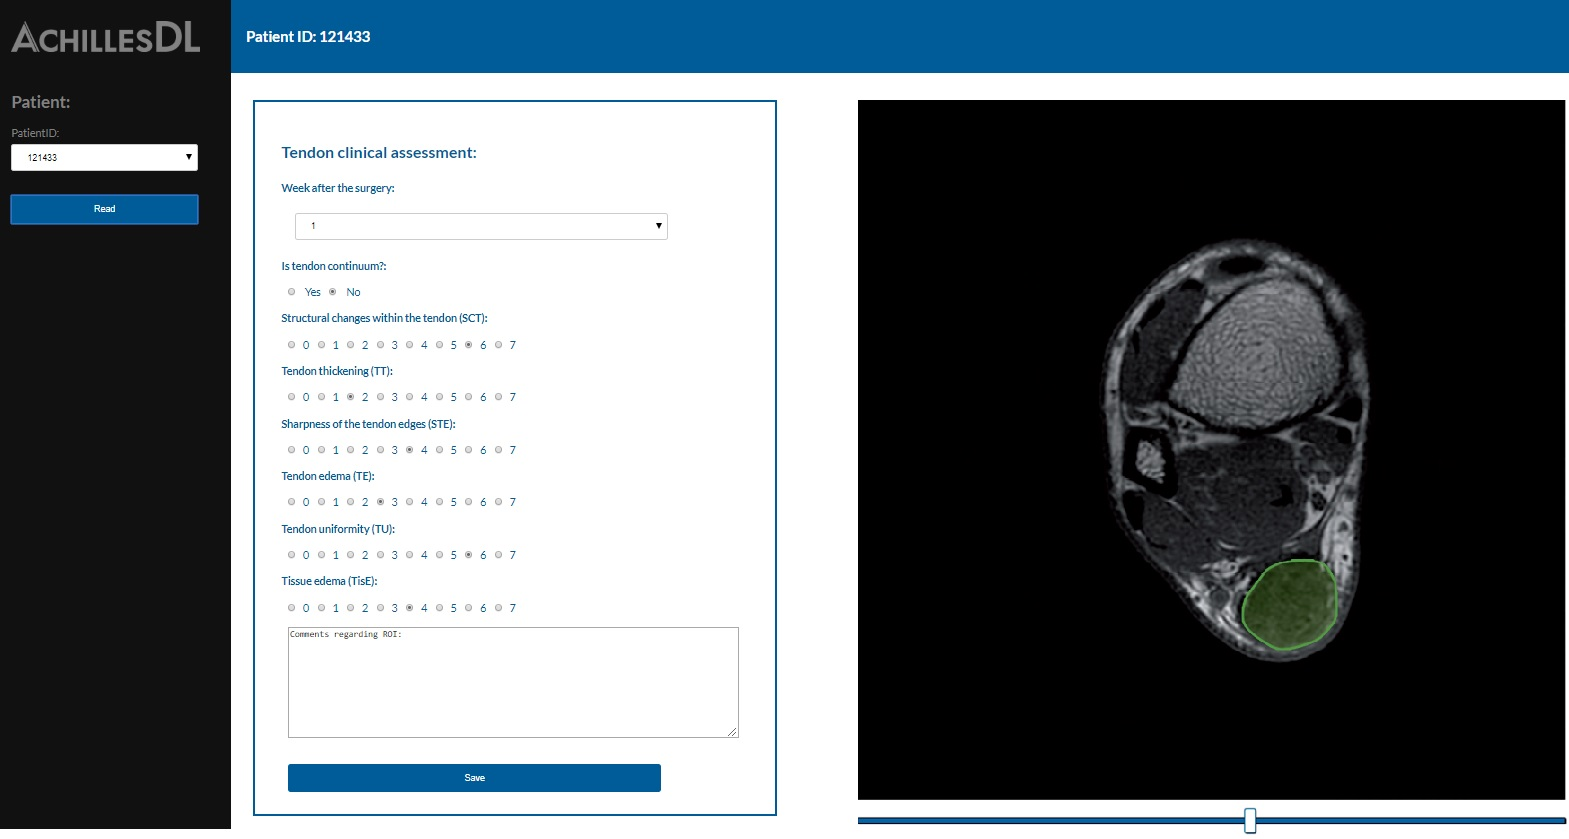
\includegraphics[width=1\textwidth]{figures/achillesDL.jpg}
	\caption{Front-end aplikacji AchillesDL przeznaczonej do oznaczania badań RM ścięgna Achillesa.}\label{fig:achillesDL}
\end{figure}
W ramach projektu START powstał rozwijany przez autora tej pracy system AchillesDL służący do intuicyjnego przeglądania i etykietowania danych radiologicznych z wykorzystaniem przeglądarki internetowej. System ten został zaprezentowany na konferencji NVIDIA GTC 2018 w San Jose, Kalifornia \cite{KapinskiGTC2018}. Front-end aplikacji można zobaczyć na Rys. \ref{fig:achillesDL}.


System umożliwia:
\begin{itemize}[noitemsep,nolistsep]
	\item wybór pacjenta i prezentację danych z bazy;
	\item wizualizację badań RM;
	\item wypełnienie i zapis ankiety omówionej w p. \ref{seq:ground-truth}.
\end{itemize}

Trwają również prace nad wizualizacją wyników oceny automatycznej wraz \linebreak ze wskazaniem w 2D i 3D obszarów zainteresowania sieci. Po wcześniejszym skontaktowaniu się z autorem tej pracy pod adresem mailowym norkap@icm.edu.pl możliwy jest dostęp do systemu poprzez stronę achillesdl.icm.edu.pl.

%%%%%%%%%%%%%%%%%%%%%%%%%%%%%%%%%%%%%%%%%%%%%%%%%%%%%%%%
\chapter{Cechy Haralicka}
\label{app:Haralick}
Poszczególne cechy Haralicka w tej pracy wyliczane są dla funkcji obrazowej przekształconej z wykorzystaniem \textit{znormalizowanej macierzy współwystępowania}: 
\begin{equation}
HP_{i,j} = \frac{HV_{i,j}}{HR}
\end{equation}
gdzie $HP$ to znormalizowana macierz współwystępowania\index{$HP$ -- znormalizowana macierz współwystępowania}, $HV$\index{$HV$ -- liczba par punktów obrazowych w oknie wyliczania macierzy współwystępowania, które mają taką samą wartość funkcji obrazowej, odległych od siebie o dystans separacji} to liczba par punktów obrazowych, które mają taką samą wartość funkcji obrazowej, odległych od siebie o pewien określony dystans wzdłuż półprostej o punkcie początkowym w $i$, $j$, nachylonej pod kątem $\alpha_h$ (tzw. dystans separacji). $HR$\index{$HR$ -- liczba wszystkich par punktów obrazowych w oknie wyliczania macierzy współwystępowania oddalonych o dystans separacji} to natomiast liczba wszystkich par oddalonych o dystans separacji. 

Z wykorzystaniem macierzy współwystępowania można zdefiniować następujących 12 cech Haralicka\index{hf1-12 -- cecha Haralicka}:
\begin{itemize}
	\item drugi moment kątowy:
	\begin{equation}
		hf_1 = \sum_i \sum_j {HP(i,j)}^2,
	\end{equation} 
	\item kontrast:
	\begin{equation}
		hf_2 = \sum_{n=0}^{N-1}n^2\left\{{\sum_{\substack{i=1\\|i-j|=n}}^{N} \sum_{j=1}^{N}} HP(i,j)\right\},
	\end{equation}  
	\item korelacja:
	\begin{equation}
		hf_3 = \frac{\sum_{i} \sum_{j}(ij)HP(i,j) - \mu_{hx}\mu_{hy}}{\sigma_{hx}\sigma_{hy}},
	\end{equation}
	gdzie $\mu_{hx}$, $\mu_{hy}$, $\sigma_{hx}$, $\sigma_{hy}$ to odpowiednio średnie i odchylenia standardowe $HP$ liczone po $x$ i $y$ (zgodnie z występowaniem w indeksie).  
	\item wariancję
	\begin{equation}
		hf_4 = \sum_i \sum_j (i - \mu_{hxy})^2 HP(i,j),
	\end{equation}
	\item odwrotny moment różnicowy
	\begin{equation}
		hf_5 = \sum_i \sum_j \frac{1}{1+(i-j)^2}HP(i,j),
	\end{equation} 
	\item sumę średnich
	\begin{equation}
		hf_6 = \sum_{i=2}^{2N}i HP_{x+y}(i),
	\end{equation} 
	gdzie:
	 \begin{equation}
	 HP_{x+y}(k) = \sum_{\substack{i=1 \\ i+j = k}^{N}} \sum_{j=1}^{N} HP(i,j)
	 \end{equation}
	\item sumę entropii
	\begin{equation}
		hf_7 = - \sum_{i=2}^{2N}HP_{x+y}(i) log(HP_{x+y}(i)),
	\end{equation} 
	\item sumę wariancji
	\begin{equation}
		hf_8 = \sum_{i=2}^{2N}(i - hf_7)^2 HP(i),
	\end{equation} 
	\item entropię
	\begin{equation}
		hf_9 =  - \sum_i \sum_j HP(i,j) log(HP(i,j)),
	\end{equation} 
	\item różnicę wariancji
	\begin{equation}
	 	hf_{10} = \sigma^2(HP_{x-y}),
	\end{equation} 
	gdzie:
	\begin{equation}
		HP_(x-y)(k) = \sum_{\substack{i=1 \\ |i-j| = k}}^{N} \sum_{j=1}^{N} HP(i,j),
	\end{equation} 	
	\item różnicę entropii
	\begin{equation}
	 hf_{11} = - \sum_{i=0}^{N-1} HP_{x-i}(i)log(HP_{x-y}(i)),
	\end{equation}
	\item maksimum prawdopodobieństwa
	\begin{equation}
	hf_12 = max(HP),
	\end{equation}
\end{itemize}
